\begin{table}[!ht]
\centering
 \begin{tabular}{c|l|l|l|l|l|}
 & UE & UW & IE & BR & SG \\
\hline
\multirow{2}{*}{UE} &  0.4 ms  & 85 ms    & 92 ms    & 150 ms &  252 ms\\
   &  994 Mbps& 164 Mbps & 242 Mbps & 53 Mbps & 86 Mbps\\
\hline
\multirow{2}{*}{UW} &          & 0.3 ms   & 155 ms   & 207 ms  & 181 ms \\
   &          & 975 Mbps & 84 Mbps  & 35 Mbps & 126 Mbps \\
\hline
\multirow{2}{*}{IE} &          &          & 0.4 ms   & 235 ms  & 350 ms  \\
   &          &          & 996 Mbps & 54 Mbps & 52 Mbps \\
\hline
\multirow{2}{*}{BR} &          &          &          & 0.3 ms  & 380 ms \\
   &          &          &          & 993 Mbps& 65 Mbps \\
\hline
\multirow{2}{*}{SG} &          &          &          &         & 0.3 ms\\
   &          &          &          &         & 993 Mbps\\
\hline
\end{tabular}
\caption{Average round trip latency and bandwidth between Amazon datacenters.}
\label{tab:roundtriplatency}
\end{table}

\section{Evaluation}
\label{ch:redblue:sect:eval}
We evaluate \gemini\ and \RBc\ using microbenchmarks and
our three case study applications.  The primary goal of our evaluation
is to determine if \RBc\ can improve latency and throughput in
geo-replicated systems. More precisely, we focus on the following
main questions:

\begin{itemize}
\item What is the impact of colors of shadow operations on user observed latency?
\item How does throughput change when varying the ratio of \red\ (strongly
consistent) shadow operations?
\item What is the prevalence of \blue\ or \red\ \shadow\ \operations\ in the three applications introduced
in the previous section?
\item How does throughput change when increasing the replication factor (i.e., the number of sites)?
\item What is the overhead of \gemini?
\end{itemize} 

\subsection{Experimental setup} 

We run experiments on Amazon EC2~\cite{AmazonEC2} using extra large virtual
machine instances located in five \dcs: US east (UE), US west (UW),
Ireland (IE), Brazil (BR), and Singapore (SG).
Table~\ref{tab:roundtriplatency} shows the average round trip latency
and observed bandwidth between every pair of \dcs.  For experiments
with fewer than 5 \dcs, new \dcs\ are added in the following order:
UE, UW, IE, BR, SG.  Unless otherwise noted, users are evenly
distributed across all sites.  Each VM has 8 virtual cores and 15GB of
RAM.  VMs run Debian 6 (Squeeze) 64 bit, MySQL 5.5.18, Tomcat 6.0.35,
and Sun Java SDK 1.6. Each experimental run lasts for 10 minutes.

\subsection{Microbenchmark}
\label{sect:micro}

%new
We begin the evaluation with a simple microbenchmark
  designed to stress the costs and benefits of partitioning
  \operations\ into \red\ and \blue\ sets.  Each user issues requests
  accessing a random record from a MyS\-QL database. Each
  request maps to a single \shadow\ \operation; we say a
  request is \blue\ if it maps to a \blue\ \shadow\ \operation\ and
  \red\ otherwise.  The offered workload is varied by adjusting the
  number of outstanding requests per user and the ratio of \red\ and
  \blue\ requests.

We run the microbenchmark experiments with a dataset consisting of 10
tables each initialized with 1,000,000 records; each record has 1 text
and 4 integer attributes.  The total size of the dataset is 1.0
GB. 

\begin{figure}[H]
\centering

\subfloat[\textsf{\Blue\ request latency for all users as number of \dcs\ increases}]{
\includegraphics[width=0.65\columnwidth]{figures/redblue/redallUserBar.pdf}
\label{fig:microallredup}
}
\hspace{2mm}
\subfloat[\textsf{\Red\ request latency for all users as number of \dcs\ increases}]{
\includegraphics[width=0.65\columnwidth]{figures/redblue/blueallUserBar.pdf}
\label{fig:microallblueup}
}
\\
\subfloat[\textsf{\Blue\ latency CDF for Singapore users as number of \dcs\ increases}]{
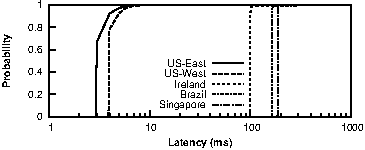
\includegraphics[width=0.65\columnwidth]{figures/redblue/thla2dcreadupdate.pdf}
\label{fig:microredup}
}
\hspace{2mm}
\subfloat[\textsf{\Red\ latency CDF for Singapore users as number of \dcs\ increases}]{
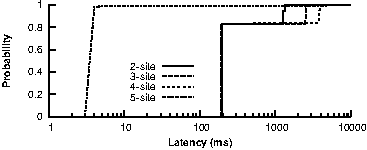
\includegraphics[width=0.65\columnwidth]{figures/redblue/thla2dcblueupdate.pdf}
\label{fig:microblueup}
}
\caption{\protect\subref{fig:microallredup} and \protect\subref{fig:microallblueup} show the average latency and standard
    deviation for \blue\ and \red\ requests issued by users in
    different locales as the number of \dcs\ is increased,
    respectively. \protect\subref{fig:microredup} and \protect\subref{fig:microblueup} show the CDF of latencies for \blue\ and
    \red\ requests issued by users in Singapore as the number of
    \dcs\ is increased, respectively.}
\label{fig:microuserbargraph}
\end{figure}

\if 0
In our microbenchmark application \changebars{users issue \operations\
 that touch a single randomly chosen object}  {we issue transactions with a single read
  or write request} in an open loop, i.e., each user has a window of
 outstanding \transactions. \changebars{Each \operation\
  is mapped to one shadow
  \transaction.  For simplicity, we label the original operations \red\ or \blue\ as well, according to the
color of their \shadow\ \operations. }{}The benchmark code allows for setting
  knobs with the ratio of read-only versus write-only \operations, and
 \blue\ versus \red\ \operations.

The dataset we used contains 10 tables\changebars{, each of which has
  the same schema consisting of 4 integer and 1 text attributes and is
  initialized with $100,000$ records. %, resulting in a $1.0$ GB
  dataset size.  }{, each of which with $100,000$ records.} The total
size of the dataset is $1.0$ GB. \changebars{}{Unless otherwise noted
  the workload does not contain any read-only requests.}
%for analysis after warm-up.}{}
%\daniel{remove the workload note and add a short note in every experiment that makes the flow more smooth}
}
\fi

\subsubsection{User observed latency}
The primary benefit of using \gemini\ to replicate a service across
multiple \dcs\ is the decrease in latency from avoiding the intercontinental round-trips as much as possible. As
a result, we first explore the impact of \RBc\ on user experienced
latency. In the following experiments each user issues a single
outstanding request at one time.
%Figure~\ref{fig:microuserbargraph} displays the average
%latency for users located in each of the five \changebars{\dcs}{data
%  centers}. 



%\changebars{In this experiment, the workloads consist of all write-only \transactions.}{}

%% \begin{figure}[t]
%% \centering
%% \subfigure[\red\ \transaction]{
%% \conferenceOnly{\includegraphics[width=0.95\columnwidth]{figures/redallUserBar.pdf}}
%% \techReportOnly{\includegraphics[width=0.7\columnwidth]{figures/redallUserBar.pdf}}
%% \label{fig:microallredup}
%% }
%% \subfigure[\blue\ \transaction]{
%% \conferenceOnly{\includegraphics[width=0.95\columnwidth]{figures/blueallUserBar.pdf}}
%% \techReportOnly{\includegraphics[width=0.7\columnwidth]{figures/blueallUserBar.pdf}}
%% \label{fig:microallblueup}
%% }
%% \caption{\changebars{Microbenchmark: + 0.1GB database}{} average latency of \blue\ and \red\ \transactions\ for users at different \dcs\ as the number of \dcs\ that replicate the service increases.}
%% \label{fig:microuserbargraph}
%% \end{figure}

Figure~\ref{fig:microuserbargraph}\subref{fig:microallredup} shows that the average
  latency for \blue\ requests is dominated by the latency between the
  user and the closest site; as expected, average latency decreases as
  additional sites appear close to the user. For example, with replicas in two sites in US, 
  users at US-East get responses in less than 10 ms, whereas users at 
  Ireland get responses of 100 ms on average, slightly above the round-trip latency of 92 ms presented
  in Table~\ref{tab:roundtriplatency}.
  Figure~\ref{fig:microuserbargraph}\subref{fig:microallblueup} shows that this trend 
  also holds for \red\ requests. The average latency and standard deviation,
  however, are higher for \red\ requests\ than for \blue\ requests. This
is because \red\ \shadow\ \operations\ can be as fast as \blue\ ones if
their primary site holds the unique red token, but will be much slower if
the site does not have that privilege.
  
Figures~\ref{fig:microuserbargraph}\subref{fig:microredup} and~\ref{fig:microuserbargraph}\subref{fig:microblueup} show the CDFs
  of observed latencies for \blue\ and \red\ requests, respectively,
  from the perspective of users located in Singapore.  The observed
  latency for \blue\ requests tracks closely with the round-trip
  latency to the closest \dc.  In the $k=2$ through $k=4$ \dc\ configurations,
  four \red\ requests from a user in Singapore are processed at the
  closest site during the one second in which the closest site holds
  the \red\ token; every fifth request must wait $k-1$ seconds for
  the token to return.  In the 5 \dc\ configuration, the local
  \dc\ also becomes a replica of the service and therefore
  a much larger number of requests (more than 300) can be processed
  while the local \dc\ holds the \red\ token.
  This changes the format of the curve, even though the
request issued immediately after the \red\ token is
released also needs to wait four seconds for the token to return.

\if 0
\changebars{
 Figure~\ref{fig:microallredup} shows that user perceived latency for
 an all \blue\ workload is dominated by the latency between the user
 and the closest site.  As expected, user perceived latency drops as
 additional sites are added to the system.  }
%old
{
\changebars{Regarding \blue\ \transactions\ , we notice that local
  users perceive a very low latency while for remote users the latency
  is dominated by the intercontinental round-trip. For example, as
  shown Figure~\ref{fig:microuserbargraph}\subref{fig:microallredup},
  with replicas in two sites in US, users at US-East get responses in
  less than 10 ms, whereas users at Ireland get responses of 100 ms in
  average, slightly above than the round-trip latency 92 ms presented
  in Table~\ref{tab:roundtriplatency}. As expected, the latency drops
  as we add more replicas to sites closer to the users.}{For
  \blue\ transactions, we observe that local users observe a very low
  latency due to close physical proximity, while the latency of remote
  users is dominated by the intercontinental round-trip. For example,
  as shown in
  Figure~\ref{fig:microuserbargraph}\subref{fig:microallredup}, with
  two data centers, users at US-East get responses from their local
  servers in less than 10 ms, while users at Ireland observe an
  average latency of 100 ms, slightly above than the round-trip
  latency 92 ms presented in Table~\ref{tab:roundtriplatency}. As
  expected, using more data centers improves user latency in some of
  the sites}.
}
%mtadone

%metanew
\changebars{}
%metaold
{
%new
\changebars{ Figure~\ref{fig:microallblueup} shows that the user
  perceived latency for an all \red\ workload is again dependent on
  the latency between the user and the closest service site, though
  the average and standard deviation are both higher than in the all
  \blue\ workload.  Both increases are driven by the time spent waiting
  for the \red\ token to return to the closest site. 
  %\MB{This is very difficult to explain and isn't clear; old text is/was dense and non-intuitive}
}
%old
{\changebars{Looking at \red\ \transactions\ in
    Figure~\ref{fig:microuserbargraph}\subref{fig:microallblueup} we
    still observe the general trend of latency improving as we
    increase the number of sites that replicate the service. However,
    there are two relevant differences between \blue\ and
    \red\ \transactions\ . First, the average latency for
    \red\ \transactions\ is higher, due to coordination across
    sites. Second, the standard deviation of the latency of
    \red\ \transaction increases as a result of using the
    \red\ token passing protocol for coordination. The results also
    show an unexpected low latency when compared to the average time
    that is required to wait for the coordination token. This is
    because the clients that issue \red\ transactions quickly fill up
    a window of pending requests while waiting for the token, but
    manage to issue many more requests when holding the token,
    therefore driving down the average latency. This effect is
    highlighted in the next set of
    graphs.}{Figure~\ref{fig:microuserbargraph}\subref{fig:microallblueup}
    shows the latency of \red\ transactions. While we still observe
    the general trend of latency improving as the number of sites that
    replicate the \changebars{service}{state} increases, there are two
    relevant differences between \blue\ and \red\ transactions. First,
    the average latency for \red\ transactions is higher, due to the
    need \changebars{of coordination}{to coordination} across sites in
    the form of passing around the \red\ token. Second, the standard
    deviation of the latency of \red\ transaction increases due to
    the same cause. The results also show an unexpectedly low latency
    when compared to the average time that is required to wait for the
    coordination token. This is because the clients that issue
    \red\ transactions quickly fill up a window of pending requests
    while waiting for the token, but manage to issue many more
    requests when holding the token, therefore driving down the
    average latency. This effect is highlighted in the next set of
    graphs.}  }
%done
}
%metadone
\fi

\subsubsection{Peak throughput}
We now shift our attention to the throughput implications
  of \RBc.  Figure~\ref{fig:micro2dcoverall1} shows a
  throughput-latency graph for a 2 \dc\ configuration and three
  workloads: 100\% \blue, 100\% \red, and a 70\% \blue/30\% \red\ mix.
  The different points in each curve are obtained by increasing the offered
  workload, which is achieved by increasing the number of
  outstanding requests per user.  
  For the mixed workload, users are partitioned into \blue\ and
  \red\ sets responsible for issuing requests of the specified color
and the ratio is a result of this configuration.

  The results in Figure~\ref{fig:micro2dcoverall1} show that increasing the
  ratio of \red\ requests degrades both latency and throughput.
In particular, the two-fold increase in throughput for the all \blue\ workload in
 comparison to the all \red\ workload is a direct consequence of the
 coordination (not) required to process \red\ (\blue) requests:
% Recall that \gemini\ enforces the total order of 
while \red\ requests can only be executed by
the site holding the \red\ token to process,
every site may independently process
 \blue\ requests.  The peak throughput of the mixed workload is
 proportionally situated between the two pure workloads.

\if 0
%old
{Next we looked at the impact of varying the
\blue\ \shadow\ \transaction\ ratio on system performance, by
measuring the \changebars{latency and throughput for write-only
  \shadow\ \transactions\ in a 2-sites deployment while we increase
  the user load. We ran three workload configurations: $100\%$ \blue,
  $100\%$ \red\ and a mix of \blue\ and
  \red\ \shadow\ \transactions\ where we split the users into two
  sets, each one responsible for issuing only one operation type,
  resulting in $70\%/30\%$ \blue/\red\ ratio. The results are shown in
  Figure~\ref{fig:micro2dcoverall} where the points in the curves
  corresponds sequentially to the same user load. We observe that
  increasing the fraction of \red\ \shadow\ \transactions\ degrades
  both latency and throughput.} {\transaction\ latency and throughput
  in a 2-data center deployment when running workloads with $100\%$
  \blue\ update transactions, $30\%$ \red\ update transactions, and
  $100\%$ \red\ update transactions. (The choice of $30\%$ was
  constrained by the fact that we wanted to split the users into two
  sets that only performed \blue\ and \red\ transactions,
  respectively, to avoid interference between the two types). The
  results in Figure~\ref{fig:micro2dcoverall} show that increasing the
  fraction of \red\ transactions degrades both latency and
  throughput. }
}
%done
\fi

%% \begin{figure}[t]
%%   \centering
%%     \conferenceOnly{\includegraphics[width=0.95\columnwidth]{figures/thla2dcredblue.pdf}}
%%     \techReportOnly{\includegraphics[width=0.7\columnwidth]{figures/thla2dcredblue.pdf}}
%%   \caption{ \changebars{Microbenchmark + 0.1GB database: throughput vs. latency graph with workloads of $100\%$ \blue, $100\%$ \red, and the mix of $70\%$ \blue\ and $30\%$ \red\ \transactions\ in a two-\dc\  setup.}{Throughput versus latency graph for the microbenchmark workload spanning two data centers when running a mix of: $100\%$ \blue, $30\%$ \red, and $100\%$ \red.} }
%%  \label{fig:micro2dcoverall}
%% \end{figure}

\begin{figure}[t]
  \centering
\includegraphics[width=0.85\columnwidth]{figures/redblue/thla2dcredblue.pdf}
  \caption{ Throughput versus latency graph for a 2 \dc\ configuration with
    varying \red-\blue\ workload mixes.}
%\changebars{Microbenchmark + 1.0GB database: throughput vs. latency graph with workloads of $100\%$ \blue, $100\%$ \red, and the mix of $70\%$ \blue\ and $30\%$ \red\ \transactions\ in a two-\dc\  setup.}{Throughput versus latency graph for the microbenchmark workload spanning two data centers when running a mix of: $100\%$ \blue, $30\%$ \red, and $100\%$ \red.} }
 \label{fig:micro2dcoverall1}
\end{figure}

\if 0
The degraded performance of the all \red\ workload is explained by
the need for cross-site coordination. In particular, in our
serialization protocol, at each point in time there is only one
\dc\ processing \red\ \transactions; the remaining ones are waiting
for the token, resulting in lower throughput and higher
latency. Introducing a mix of \blue\ \changebars{and
  \red\ \transactions}{transactions} sites run concurrent \dcs\ to
process transactions of one or both types at each moment, thus
increasing throughput. Moving to an \blue\ workload leads to a further
improvement in latency due to the possibility of executing
\transactions\ immediately without coordination. This highlights our
main motivation of running as many \blue\ \transactions\ as possible,
provided it does not undermine consistency.
\fi 

%metanew dropping scaling with datacenters
\if 0
\changebars{}
%metaold
{
%new
\changebars{Figure~\ref{fig:microScaleOverall} shows the
  throughput-latency curves for 2-5 \dc\ configurations processing a
  70 \blue/30 \red\ mixed workload.  We observe that both throughput
  and average latency improve as additional \dcs\ are added.  The
  latency improvement is the natural consequence of reducing the
  average distance between users and datacenters.  The throughput
  improvement is driven by the ability of \dcs\ to independently
  process \blue\ requests.
}{\subsubsection{Scalability with the number of sites}
}}
%metadone

%new dropping figure on scalability
\changebars{}
%old
{
\begin{figure}[t]
  \centering
  \conferenceOnly{\includegraphics[width=0.95\columnwidth]{figures/thla2dc3dc4dc5dcreadwrite.pdf}}
  \techReportOnly{\includegraphics[width=0.7\columnwidth]{figures/thla2dc3dc4dc5dcreadwrite.pdf}}
  \caption{\changebars{Microbenchmark:}{Microbenchmark} throughput
    vs.\ latency curves while varying the geo-replication factor from
    2 to 5 \dcs. }
 \label{fig:microScaleOverall}
\end{figure}
}
%done

%metanew
\changebars{

}
%metaold
{
To evaluate the scalability of \gemini\ with the number of geographic
locations of data, we deployed \gemini\ across 2 to 5 data centers and
measured both throughput and latency. In this experiment we fix the
mix of read/write and \blue/\red\ \changebars{\transactions}{} in a
balanced way that conservatively reflects our experience with
\changebars{the case studies}{real applications}, to 50/50 and 90/10,
respectively.

In Figure~\ref{fig:microScaleOverall} we plot the throughput and
latency for the four deployments. The different points in the same
curve correspond to a varying client load, which generates a higher
throughput but slower access times as the system saturates
\daniel{define it more precisely: how it varies?}. \changebars{These
  results unveils a trend, showing that \gemini\ scales well as the
  number of data-centers increases. Furthermore, despite the main
  benefit of \gemini\ be in latency, we can also observe a substantial
  improvement in system throughput following the same trend}{The
  results show that the performance of our architecture scales well as
  the number of data centers increases. Furthermore, despite the main
  benefit of \gemini\ being transaction latency, we can also
  substantially improve system throughput as the geo-replication
  factor increases,} due to two main reasons.  
%new
\changebars{The first reason is a direct consequence of latency
  improvement: as we add more data-centers close to users we amortize
  latency time in all transactions, therefore the transactions run
  faster and we end up with more transactions in the same experiment
  period. Second, we can also observe a shift in saturation wall, that
  is explained by the fact that we increase the capacity of the system
  as we add more data-centers to process users requests, enabling more
  local transactions (read-only) to be executed before the saturation
  point}
%old
{First, read-only transactions do not need to be propagated to
  remote sites. Second, it is cheaper for a data-center to process the
  shadow \transaction required for remote execution than to perform
  both the initial and the shadow transaction.}
%done
\daniel{the explanation is broken because microbenchmark read-only
  transactions were not being propagated before add more data-centers
  hence it did not change therefore cannot be the reason to improve
  the throughput specially when the system is not saturated. The
  second one is also broken because we already split the work of
  executing initial/generator transactions among more instances of
  proxies and the system is not saturated}
}
%metadone
\fi

\subsection{Case studies:  TPC-W and RUBiS}
Our microbenchmark experiments indicate that \RBc\ instantiated with
\gemini\ offers latency and throughput benefits in geo-replicated
systems with sufficient \blue\ \shadow\ \operations. Next, we evaluate \gemini\ using TPC-W and RUBiS.

\subsubsection{Configuration and  workloads}
In all case study experiments a single \dc\ configuration
corresponds to the original unmodified code with users distributed
amongst all five sites.  Two through five \dc\ configurations
correspond to the modified \RBct\ systems running on top of \gemini.
When necessary, we modified the provided user emulators so that each
user maintains $k$ outstanding requests and issues the next request as
soon as a response is received.

\paragraph{TPC-W.}
TPC-W~\cite{TPC-Wv18} defines three workload mixes
differentiated by the percentage of client requests related to making
purchases: browsing (5\%), shopping (20\%), ordering (50\%). The
dataset is generated with the following TPC-W
parameters: 50 EBS and $10,000$ items.  

%We specifically highlight the performance of the doBuyConfirm,
%discussed in detail in \S~\ref{sect:casetpcw}, and doCart, which adds
%items to and removes items from a specific shopping cart, requests.
%doCart always maps to a \red\ \shadow\ \operation. doBuyConfirm can
%map to either a \blue\ or \red\ \shadow\ \operation; in our
%experiments it is \red\ 98\% of the time.

\paragraph{RUBiS.}
RUBiS defines two workload mixes: browsing, exclusively comprised of
read-only interactions, and bidding, where $15\%$ of user
interactions are updates. We evaluate only the bidding mix. The RUBiS
database contains $33,000$ items for sale, 1 million users, $500,000$
old items and is $2.1$ GB in total.

%We specifically highlight the performance of StoreBid, which places a
%bid on an item, and StoreBuyNow, which purchases an item for the
%buyout price.  StoreBid always maps to a \blue\ \shadow\ \operation.
%StoreBuyNow may map to either a \blue\ or \red\ \shadow\ \operation;
%in our experiments it is \red\ 99\% of the time.

\subsubsection{Prevalence of \blue\ and \red\ \shadow\ \operations}

\begin{table}[t]
\centering
\begin{tabular}{|l||c|c||c|c|}
\hline
& {\Blue\  } &  {\Red\ } & read-only  & update\\
\hline
\hline
TPC-W shop&  99.2 & 0.8 &85 & 15\\
\hline
TPC-W browse &  99.5 & 0.5 & 96 & 4 \\
\hline
TPC-W order & 93.6  & 6.4 & 63 & 37 \\
\hline
RUBiS bid & 97.4 & 2.6 & 85 & 15\\
\hline
\end{tabular}
\caption{Proportion of \blue\ and \red\ \shadow\ \transactions\ and
  read-only and update requests in TPC-W and RUBiS workloads at
  runtime.}
\label{tab:mix}
\end{table}


Table~\ref{tab:mix} shows the distribution of \blue\ and
\red\ \shadow\ \operations\ during the execution of the TPC-W and RUBiS
workloads.  The results show that TPC-W and RUBiS exhibit sufficient
\blue\ \shadow\ \operations\ for it to be likely that we can exploit
the potential of \RBc.
%for \RBc\ to be a promising technique for
%building systems that are fast as possible and consistent when
%necessary.

\begin{figure}[H]
\centering
\subfloat[\textsf{TPC-W doCart}]{
\includegraphics[width=0.65\columnwidth]{figures/redblue/doCart/doCartallUserBar.pdf}
\label{fig:tpcwdocart}
}
\hspace{2mm}
\subfloat[\textsf{TPC-W doBuyConfirm}]{
\includegraphics[width=0.65\columnwidth]{figures/redblue/doBuyConfirm/doBuyConfirmallUserBar.pdf}
\label{fig:tpcwdobuyconfirm}
}
\\
\subfloat[\textsf{RUBiS StoreBid}]{
\includegraphics[width=0.65\columnwidth]{figures/redblue/storeBidallUserBar.pdf}
\label{fig:rubisStoreBid}
}
\hspace{2mm}
\subfloat[\textsf{RUBiS StoreBuyNow}]{
\includegraphics[width=0.65\columnwidth]{figures/redblue/storeBuyNowallUserBar.pdf}
\label{fig:rubisStoreBuyNow}
}
\caption{Average latency for selected TPC-W and RUBiS user
  interactions. \Shadow\ \operations\ for doCart and StoreBid are
  always \blue; for doBuyConfirm and StoreBuyNow they are \red\ 98\%
  and 99\% of the time respectively.}
\label{fig:tpcwrubisuserbargraph}
\end{figure}

\subsubsection{User observed latency}
We first explore the per request latency for a set of exemplar
\blue\ and \red\ requests from TPC-W and RUBiS.  For this round of experiments, each
\dc\ hosts a single user issuing one outstanding request to the
closest \dc.

From TPC-W we select doBuyConfirm (discussed in detail in
Section~\ref{ch:redblue:sect:casetpcw}) as an exemplar for \red\ requests and doCart
(responsible for adding/removing items to/from a shopping cart) as an
exemplar for \blue\ requests; from RUBiS we identify StoreBuyNow
(responsible for purchasing an item at the buyout price) as an
exemplar for \red\ requests and StoreBid (responsible for placing a
bid on an item) as an exemplar for \blue\ requests.  Note that
doBuyConfirm and StoreBid can produce either \red\ or
\blue\ \shadow\ \operations; in our experience they produce
\red\ \shadow\ \operations\ 98\% and 99\% of the time respectively.

Figures~\ref{fig:tpcwrubisuserbargraph}\subref{fig:tpcwdocart} and~\ref{fig:tpcwrubisuserbargraph}\subref{fig:rubisStoreBid} show
that the latency trends for \blue\ \shadow\ \operations\ are consistent
with the results from the microbenchmark---observed latency is directly
proportional to the latency to the closest \dc.  The raw latency
values are higher than the round-trip time from the user to the
nearest \dc\ because processing each request involves sending one or
more images to the user.
%; delivery time per image is one round-trip.

For \red\ requests, Figures~\ref{fig:tpcwrubisuserbargraph}\subref{fig:tpcwdobuyconfirm} 
and~\ref{fig:tpcwrubisuserbargraph}\subref{fig:rubisStoreBuyNow} show
that latency and standard deviation both
increase with the number of \dcs.  The increase in standard deviation
is an expected side effect of the simple scheme that \gemini\ uses to
exchange the \red\ token and is consistent with the microbenchmark
results.  Similarly, the increase in average latency is due to the
  fact that the time for a token rotation increases, together with the
  fact that \red\ requests are not frequent enough that several
  cannot be slipped in during the same token holding interval.  We
note that the token passing scheme used by \gemini\ is simple and
we leave as future work the implementation of a more sophisticated
scheme like Paxos~\cite{Lamport1998Paxos} for
regulating \red\ \shadow\ \operations.

\begin{figure*}[th!]
  \centering
\subfloat[\textsf{TPC-W shopping mix}]{
\includegraphics[width=0.88\columnwidth]{figures/redblue/thlatpcw1dc2dc3dc4dc5dc.pdf}
 \label{fig:tpcwoverall}
}
\\
\par\bigskip
\subfloat[\textsf{RUBiS bidding mix}]{
 \includegraphics[width=0.88\columnwidth]{figures/redblue/thla1dc2dc3dc4dc5dcRUBiSGemini.pdf}
  \label{fig:rubisoverall} 
}
\caption{Throughput versus latency for the TPC-W shopping mix and
  RUBiS bidding mix. The 1-dc line corresponds to the original code;
  the 2/3/4/5-dc lines correspond to the \RBct\ system variants.}
\label{fig:throughputscaling}
\end{figure*}

\subsubsection{Peak throughput}
We now shift our attention to the throughput afforded by our
\RBct\ versions of TPC-W and RUBiS, and how it scales with the
number of sites. For these experiments we vary the
workload by increasing the number of outstanding requests maintained by
each user.  Thr\-oughput is measured according to interactions per
second, a metric defined by TPC-W to correspond to user requests per
second.

Figure~\ref{fig:throughputscaling} shows throughput and latency for
the TPC-W shopping mix and RUBiS bidding mix as we vary the number of
\dcs.  In both systems, increasing the number of \dcs\ increases
peak throughput and decreases average latency.  The decreased latency
results from situating users closer to the \dc\ processing their
requests.  The increase in throughput is due to
processing \blue\ and read-only operations at multiple \dcs, given
that processing their side effects is relatively inexpensive.  The
speedup for a 5 \dc\ \gemini\ deployment of TPC-W is
3.7x against the original code for the shopping mix; the
5 \dc\ \gemini\ deployment of RUBiS shows a speedup of 2.3x.  


\begin{figure}[t!]
  \centering
\includegraphics[width=0.85\columnwidth]{figures/redblue/thla2dcTPCWallmixes.pdf}
  \caption{TPC-W: Throughput vs. latency graph for TPC-W with \gemini\ spanning two \dcs\ when running the three workload mixes. }
 \label{fig:tpcw2dcallmixes}
\end{figure}


Figure~\ref{fig:tpcw2dcallmixes} shows the throughput and latency
graph for a two \dc\ configuration running the TPC-W browsing,
shopping, and ordering mixes.  As expected, the browsing mix, which has
the highest percentage of \blue\ and read-only requests, exhibits the
highest peak throughput, and the ordering mix, with the lowest
percentage of \blue\ and read-only requests, exhibits the lowest peak
throughput. 
%For all workloads,
%\RBc\ improves latency by executing \operations\ closer to the user
%and improves throughput by not having to replicate all of the work,
%namely the execution of \initial\ \operations\ and
%read-only requests.

\subsection{Case study: Quoddy}
Quoddy differs from TPC-W and RUBiS in one crucial way: it has no
\red\ \shadow\ \operations.  We use Quod\-dy to show the full
power of \RedBlue\ geo-rep\-li\-ca\-tion.

Quoddy does not define a benchmark workload for testing purposes.  Thus we
design a social networking workload generator based on the measurement
study of Benevenuto et al.~\cite{Benevenuto2009Character}.  In this
workload, 85\% of the interactions are read-only page loads and 15\% of
the interactions include updates, e.g., request friendship, confirm
friendship, or update status.  Our test database contains 200,000
users and is 2.6 GB in total size.

In a departure from previous experiments, we run only two
configurations.  The first is the original Quoddy code in a
single \dc.  The second is our \gemini\ based \RBct\ version
replicated across 5 \dcs.  In both configurations, users are
distributed in all 5 regions.

Figure~\ref{fig:quoddyCDF} shows the CDF of user experienced latencies
for the addFriend operation. All \gemini\ users experience latency
comparable to the local users in the original Quoddy deployment; a
dramatic improvement for users not based in the US East region.  The
significantly higher latencies for remote regions are associated with
the images and javascripts that Quoddy distributes as part of processing the addFriend request.

\begin{figure}[t]
\centering
\includegraphics[width=0.85\columnwidth]{figures/redblue/thlaquoddyComparisonAll.pdf}
\caption{User latencies CDF for the addFriend request in single site Quoddy
   and 5-site \gemini\ deployments.}
\label{fig:quoddyCDF}
\end{figure}

                                                                                                                               

\subsection{\gemini\ overheads}


\gemini\ is a middleware layer that interposes between the
applications that leverage \RBc\ and a set of database systems where
data is stored. We evaluate the performance overhead imposed by our
prototype by comparing the performance of a single
\dc\ \gemini\ deployment with the unmodified TPC-W and RUBiS systems
directly accessing a database.
For this experiment we locate all users in the same \dc\ as the service.



\begin{table}[t]
\small
\centering
\begin{tabular}{|c|c|c|c|c|}
\hline
& \multicolumn{2}{c}{\textbf{TPC-W shopping}} & \multicolumn{2}{|c|}{\textbf{RUBiS biding}} \\
\cline{2-5}
& Original & Gemini & Original & Gemini\\
\hline
\hline
\specialcell{Thput. (inter/s)} &  409 & 386 & 450 & 370 \\
\hline
\specialcell{Avg. latency} & 14 ms & 15 ms & 6 ms & 7 ms \\
\hline
\end{tabular}
\caption{Performance comparison between the original code and the \gemini\ version for both TPC-W and RUBiS within a single site.}
\label{tab:performanceoverhead}
\end{table}

Table~\ref{tab:performanceoverhead} presents the peak throughput and
average latency for the TPC-W shopping and RUBiS bidding mixes. The peak
throughput of a single \dc\ \gemini\ deployment is between 82\% and 94\%
of the original and \gemini\ increases
latency by 1ms per request.  




%% \paragraph{Latency of individual requests.} 
%% To distinguish between the latency of \blue\ and \red\ transactions,
%% we separated the latency of two individual transactions of the system:
%% doCart (\blue) and \changebars{doBuyConfirmDecre}{doBuyConfirm}
%% (\red).  The results are shown in Figure~\ref{fig:tpcwuserbargraph}.

%% Similarly to the microbenchmarks, client latency for the \blue\ doCart
%% interaction (shown in Figure~\ref{fig:tpcwuserbargraph}\subref{fig:tpcwdocart}) decreases as
%% the latency to the closest replica decreases. We noticed, however,
%% that the latency observed by remote clients is a few times larger than
%% the round-trip latency between them and their nearest server. The
%% reason is that the doCart interaction performs the delivery of some
%% images (interspersed sequentially with transaction execution), and for
%% large images the effect of bandwidth differences between clients becomes
%% noticeable.

%% For the \red\ transaction that completes a purchase,
%% Figure~\ref{fig:tpcwuserbargraph}\subref{fig:tpcwdobuyconfirm} shows
%% that the transaction latency increases as the number of data centers
%% increases, with also an increase in the standard deviation. This is a
%% consequence of the fact that cross-site coordination gets more
%% expensive with the increase in the number of data centers,
%% particularly given that we employed a fixed timeout for passing the
%% coordination token between sites. In this case, since this
%% \red\ transaction occurs sporadically, it needs to wait on average
%% about half the token rotation period (or about 2 seconds for a five
%% site deployment).

%% \begin{figure}[t]
%%   \centering
%%   \conferenceOnly{\includegraphics[width=1.0\columnwidth]{figures/thla2dcTPCWallmixes.pdf}}
%%   \caption{TPC-W: Throughput vs. latency graph for TPC-W with \gemini\ spanning two \dcs\ when running the three workload mixes. }
%%  \label{fig:tpcw2dcallmixes}
%% \end{figure}



%% \paragraph{Overall benchmark performance.} In Figure~\ref{fig:tpcwoverall} we plot throughput vs.\ latency curves for the TPC-W benchmark. We plot five curves corresponding to deployments with replicas in one through five data centers. The results confirm that the system scales well with the number of geo-replication sites, reaching a maximum of 1500 interactions per second with replicas in five data centers, which is 3.67$x$ of the peak throughput achieved by running original TPC-W within a single site.



%% \begin{figure}[t]
%%   \centering
%%   \conferenceOnly{\includegraphics[width=1.0\columnwidth]{figures/thlatpcw1dc2dc3dc4dc5dc.pdf}}
%%   \techReportOnly{\includegraphics[width=0.75\columnwidth]{figures/thlatpcw1dc2dc3dc4dc5dc.pdf}}
%%   \caption{ \changebars{TPC-W: Throughput vs. latency graph of the
%%       original TPC-W in one data-center and TPC-W with
%%       \gemini\ spanning in 2 through 5 data-centers.}{Throughput and
%%       latency graph of the original TPC-W within one data center and
%%       TPC-W running on the top of \gemini\ systems and spanning 2
%%       through 5 datacenters.} }
%%  \label{fig:tpcwoverall}
%% \end{figure}

%% \subsubsection{RUBiS}
%% \label{sect:rubis}
%% RUBiS defines two workload mixes: a browsing mix consisting only of
%% read-only interactions and a bidding mix that includes $15\%$ of
%% updates. Our evaluation uses only the more general bidding mix. The
%% RUBiS database contains $33,000$ items for sale, 1 million users,
%% $500,000$ old items and is $2.1$ GB in total. For each experiment,
%% emulated clients continuously issue requests to the auction site, for
%% a time period of 10 minutes without think time.  We used the same
%% deployment conditions as in the TPC-W experiments.

%% \paragraph{Latency of individual transactions:} We report in
%% Figure~\ref{fig:rubisuserbargraph} the average latency observed by
%% users for two RUBiS interactions: \emph{storeBid} %
%% (Figure~\ref{fig:rubisuserbargraph}\subref{fig:rubisStoreBid}) and
%% \emph{storeBuyNow}.  %
%% (Figure~\ref{fig:rubisuserbargraph}\subref{fig:rubisStoreBuyNow}).
%% The \emph{storeBid} interaction contains a single \blue\ transaction
%% that puts a bid on an item, while the \emph{storeBuyNow}
%% interaction represents a more demanding operation, since it
%% includes a \red\ transaction that purchases items and updates the
%% stock.


%% As before, we observe significant latency benefits for
%% \blue\ transactions as we increase the number of data
%% centers. Furthermore, when interactions need to run a
%% \red\ transaction as in the case of {\tt storeBuyNow}, increasing
%% the number of data centers highlights the costs of cross-data
%% centers coordination. In this case the average latency of
%% \red\ transaction is slightly lower than in TPC-W because the
%% higher prevalence of \red\ transactions makes it more likely that
%% two or more \red\ transactions from the same sequence are executed
%% while holding the token (and thus the ones after the first one do
%% not wait).

% Additionally, we explore the impact of varying blue token timeout on the blue transaction latency. The outcome shows that shrinking the timeout improves the average latency of blue transactions.

%Similar to the TPC-W results, for the red interactions, using
%\gemini\ to replicate services across data centers will significantly
%improve the user observed latency. For example, moving from 2-data
%center to 5-data center, the \emph{storeBid} interaction latency
%observed by users at AG (Singapore) is dramatically changed from
%449.18 ms to 9.22 ms in average, and drops by $98.9\%$. Due to the
%blue token passing scheme, the average latency of \emph{storeBuyNow}
%observes a high standard deviation. Moreover, compared to the results
%of microbenchmark, the blue interaction average latency is much
%higher. The reason for this difference is that blue RUBiS
%interactions come into the system sparsely, while the blue
%microbenchmark interactions arrive intensively. Thus, the percentage
%of blue interactions for waiting in RUBiS is much higher than the one
%in microbenchmark. At the end, as we deployed RUBiS code in more data
%centers, the average latency of \emph{storeBuyNow} becomes larger,
%since the time of waiting for blue token gets longer.

%\rodrigo{I did not understand the following explanation: ``Moreover,
%compared to the results of microbenchmark, the blue interaction
%average latency is much higher. The reason for this difference is
%that blue RUBiS interactions come into the system sparsely, while the
%blue microbenchmark interactions arrive intensively. Thus, the
%percentage of blue interactions for waiting in RUBiS is much higher
%than the one in microbenchmark. At the end, as we deployed RUBiS code
%in more data centers, the average latency of \emph{storeBuyNow}
%becomes larger, since the time of waiting for blue token gets
%longer.''}

%\cheng{I want to explain why the average latency for blue
%transactions in RUBiS gets higher when the number the data centers
%increases, compared to the microbenchmark. The reason is that we have
%users in the microbenmark always issuing blue transactions in an open
%loop and the RUBiS doesn't. RUBiS selects blue transactions according
%to its probability table. Thus, there are fewer blue transactions in
%RUBiS than the microbenchmark. In addition, for the microbenmark,
%once the blue transaction is granted to a data center, its local blue
%users will issue a lot of blue transactions, which is more than the
%blue transactions that wait for the blue token. The majority fast
%blue transactions offset the delay introduced by the minority slow
%blue transactions. However, this doesn't hold in either RUBiS or
%TPC-W.}

%% \paragraph{Overall benchmark performance:} As shown in Figure~\ref{fig:rubisoverall}, the benchmark throughput scales well as we add geo-replication sites. In particular, the throughput scales from $450$ interactions per second in one site to $1,500$ interactions per second with five sites, an improvement of $233\%$.
%% % In addition to improve on latency provided to users, redblue consistency and \gemini\ are able to offer higher throughput. The latency and throughput graph for all deployment plans are shown in Figure~\ref{fig:rubisoverall}. The throughput of the three-site RUBiS with \gemini\ reaches 956 interactions per second and is $1.41x$ of the throughput of two-site. Remarkably, the throughput of the four-site RUBiS with \gemini\ is 1200 interactions per second and roughly $2x$ of the throughput of two-site. Moreover, the peak throughput of the five-site experiment is roughly 1500 interactions per section, which has been improved $123.9\%$, compared to the two-site one. 

%% \begin{figure}[t]
%% \centering
%% \conferenceOnly{\includegraphics[width=0.95\columnwidth]{figures/thla1dc2dc3dc4dc5dcRUBiSGemini.pdf}}
%% \techReportOnly{\includegraphics[width=0.7\columnwidth]{figures/thla1dc2dc3dc4dc5dcRUBiSGemini.pdf}}
%% \caption{Throughput vs.\ latency graph of the original RUBiS within one data center and RUBiS running on the top of \gemini\ spanning 2 through 5 data centers.}
%% \label{fig:rubisoverall}
%% \end{figure}

%% \subsection{Quoddy}
%% \daniel{we want to compare the best quoddy result with the the 5 dc
%%   setup. in this case, adding remote users to 1-dc will on increase
%%   the average latency and make original quoddy look bad. What we what
%%   to highlight that we are very close to quoddy best scenario, with
%%   the increased capacity and users across the globe in gemini
%%   scenario; therefore it is a fair comparison}

%% \paragraph{Quoddy.}
%% Quoddy does not define any benchmark workloads for testing purposes.
%% We design a social networking workload generator based on the
%% measrement study of Benevenuto et al.~\cite{Benevenuto09Character}.
%% In this workload 85\% of the interactions are read-only page loads and
%% 15\% of the interactions include updates, e.g., request friendship,
%% confirm friendship, or update status.  Our test database contains
%% 200,000 users and is 2.6 GB in total size.


%%  Unlike the two previous
%% case studies, the Quoddy social network does not come associated with
%% a benchmark specification that defines the application workload.
%% Therefore, we designed a workload generator for driving the user
%% behaviors.  The workload comprises of $85\%$ read-only interactions,
%% such as profile browsing actions and user searching, and $15\%$
%% read/write interactions including friendship requests/confirm and
%% status updates. These numbers are inspired on the results of a
%% measurement study of several social networking sites like Okurt,
%% MySpace and LinkedIn~\cite{Benevenuto09Character}.  The database
%% contains 200,000 users and is 2.6 GB in total. For each experiment,
%% the emulated users issue requests to the server for 10 minutes without
%% think time.

%% \begin{figure}[t]
%% \centering
%% \conferenceOnly{\includegraphics[width=0.95\columnwidth]{figures/thlaquoddyComparisonAll.pdf}}
%% \techReportOnly{\includegraphics[width=0.7\columnwidth]{figures/thlaquoddyComparisonAll.pdf}}
%% \caption{Distribution of latencies for addFriend interaction in Quoddy with the single site and
%% \gemini\ 5-site deployment.}
%% \label{fig:quoddyCDF}
%% \end{figure}

%% We only run Quoddy in a single data center and Quoddy with \gemini\ 
%% replicated across five data center experiments to examine the distribution 
%% of latency for different interactions. %\changebars{Unlike the deployment
%% %plans in TPC-W and RUBiS, the single data center Quoddy experiment only has local users,
%% %instead of additionally having remote users.}{Both deployment plans only have local users.} %We aggregate data from 
%% %users \changebars{}{at the five data centers}, and plot 
%% The latency CDF graph for the addFriend interaction is shown in Figure~\ref{fig:quoddyCDF}.
%% As can be seen, in the five data center case, 
%% all users observe almost the same latency as the one observed by local users at in the 
%% single data center experiment, even if Gemini servers are processing transactions 
%% received from other data centers also. The reason why Gemini impose no additional 
%% overhead is because all transactions encoded in interactions are \blue\ and thus processed locally.
%% The latency of the interaction is mostly due to the sequentially download of other resources, such as images.

%% %\rodrigo{Did not modify this paragraph, I think it's still in flux:}
%% %\cheng{Yes, we are working on this part.}
%% %Figure~\ref{} shows the throughput and latency numbers for Quoddy running on the top of \gemini\ and being replicated from 2 data centers to 5 data centers. As can be seen, the throughput has been improved significantly and the average latency has been reduced remarkably, as the number of data centers hosting service increases. In addition to the throughput and latency, we investigate evoluation of the user observed latency when we change the configuration from 2 data centers to 5 data centers. We find that the user observed latency is dramatically improved similarly to the red transactions presented in TPC-W and RUBiS. For example, users in Singapore observe xxx ms latency for read-info transactions in the two data center cases, and xxx ms latency in the five data center case. 

%% \subsection{Overhead of \gemini}


%% \gemini\ is implemented as a middleware layer that interposes between
%% the applications that leverage \RBc\ and a set of database systems
%% where data is stored. Next we evaluate the performance overhead that
%% is introduced by our system. For this, we compare the performance of a
%% single data center deployment of \gemini\ against a baseline
%% consisting of the applications directly accessing database via an unmodified JDBC driver.

%% %To support the redblue consistency model, we built a middle-tier (including coordinator, data writer and proxy library) to the traditional two-tier system architecture, in which application servers are connected to database directly via a JDBC driver. This new tier might lead to a performance drop. In order to understand how much overhead our new design introduces, we ran experiments of both the original code of two benchmarks and their redblue version with a single data center and local users.

%% %\begin{figure}[h!]
%% %\centering
%% %\subfigure[Throughput]{
%% %\includegraphics[width=0.45\columnwidth]{figures/overheadBar.pdf}
%% %\label{fig:thptOverhead}
%% %}
%% %\subfigure[Average latency]{
%% %\includegraphics[width=0.45\columnwidth]{figures/latencyOverheadBar.pdf}
%% %\label{fig:latencyOverhead}
%% %}
%% %\caption{Performance comparison between the original code and the \gemini\ version for both TPC-W and RUBiS within a single site.}
%% %\label{fig:overhead}
%% %\end{figure}

%% \begin{table}[t]
%% \small
%% \centering
%% \begin{tabular}{|c|c|c|c|c|}
%% \hline
%% & \multicolumn{2}{c}{\textbf{TPC-W}} & \multicolumn{2}{|c|}{\textbf{RUBiS}} \\
%% \cline{2-5}
%% & Original & Gemini & Original & Gemini\\
%% \hline
%% \hline
%% \specialcell{Thput. (inter/s)} &  409 & 386 & 450 & 370 \\
%% \hline
%% \specialcell{Avg. latency} & 14 ms & 15 ms & 6 ms & 7 ms \\
%% \hline
%% \end{tabular}
%% \caption{Performance comparison between the original code and the \gemini\ version for both TPC-W and RUBiS within a single site.}
%% \label{tab:performanceoverhead}
%% \end{table}

%% We compare both the peak throughput and average latency, and present
%% the results in Table~\ref{tab:performanceoverhead}.  \gemini\ achieves
%% $94.4\%$ and $82.2\%$ of the throughput of the original code, for
%% TPC-W and RUBiS respectively. In addition to this modest drop in
%% throughput, \gemini\ induces a latency that is, on average, 1 ms
%% higher per transaction when compared to the original benchmarks. This
%% shows that \gemini\ introduces modest overheads, likely worth the
%% performance benefits in geo-replicated deployments.

%%deployment of TPC-W and RUBiS is only 1 ms slower than the average latency of their original version. Although \gemini\ adds modest overhead to the original code with a single data center, it will make the original system more scalable by replicating it across multi-data centers.



%% %%%%%%%%%%%%%%%%%%%% round 2



%% \subsection{Application benchmarks (case studies)}
%% %Based on the results associated with the microbenchmark, we already saw the benefits gained when we use \gemini\ system to replicate data across multi-data centers. Next, we will show that \gemini\ also achieves good performance in the two application benchmarks: TPC-W and RUBiS.
%% Next we use our case studies to evaluate the system with application-level benchmarks.

%% \subsubsection{TPC-W}
%% \label{sect:tpcw}
%% TPC-W~\cite{TPC-Wv18} defines three workload mixes
%% differentiated by the percentage of client requests related to making
%% purchases: browsing (5\%), shopping (20\%), ordering (50\%). The
%% dataset is generated with the following TPC-W configuration
%% parameters: 50 EBS and $10,000$ items.  

%% For TPC-W experiments emulated clients issue requests for 10 minutes
%% with no think time.  We vary the offered workload by increasing the
%% number of outstanding requests maintained by each client.  One
%% \dc\ configurations correspond to the original TPC-W server with
%% clients in all regions; multiple \dc\ configurations use our
%% \RBct\ modifications and \gemini\ prototype.


%% \paragraph{Latency of individual transactions.}
%% We first 

%%  To distinguish between the latency of \blue\ and \red\ transactions, we separated the latency of two individual transactions of the system: doCart (\blue) and doBuyConfirm (\red).%\cheng{need to change, interaction is not red or blue, instead, transaction} 
%% The results are shown in Figure~\ref{fig:tpcwuserbargraph}.

%% % The main goal of \gemini\ is to offer low latency for users by allowing red transactions to be processed locally. In order to understand the evolution of user observed latency when the deployment plan changes, we further show in Figure~\ref{fig:tpcwuserbargraph} average latency for different interactions user observed at different data centers. Due to the space limitation, we only present two interactions: 

%% \begin{figure}[t]
%% \centering
%% \subfigure[doCart]{
%% \conferenceOnly{\includegraphics[width=0.95\columnwidth]{figures/doCart/doCartallUserBar.pdf}}
%% \techReportOnly{\includegraphics[width=0.7\columnwidth]{figures/doCart/doCartallUserBar.pdf}}
%% \label{fig:tpcwdocart}
%% }
%% \subfigure[doBuyConfirm]{
%% \conferenceOnly{\includegraphics[width=0.95\columnwidth]{figures/doBuyConfirm/doBuyConfirmallUserBar.pdf}}
%% \techReportOnly{\includegraphics[width=0.7\columnwidth]{figures/doBuyConfirm/doBuyConfirmallUserBar.pdf}}
%% \label{fig:tpcwdobuyconfirm}
%% }
%% \caption{Average latency for two system transactions: the doCart interaction shown in \subref{fig:tpcwdocart} is \blue, and the doBuyConfirm interaction shown in \subref{fig:tpcwdobuyconfirm} is \red.
%% %. \textbf{Note} that the first bar cluster represents a single-datacenter original version of TPC-W. The remaining four bar clusters refer to the redblue consistent version of TPC-W. The doCart interaction shown in \subref{fig:tpcwdocart} is red, and the buy confirm interaction shown in \subref{fig:tpcwdobuyconfirm} is blue.
%% }
%% \label{fig:tpcwuserbargraph}
%% \end{figure}

%% Similarly to the microbenchmarks, client latency for the \blue\ doCart
%% interaction (shown in Figure~\ref{fig:tpcwuserbargraph}\subref{fig:tpcwdocart}) decreases as
%% the latency to the closest replica decreases. We noticed, however,
%% that the latency observed by remote clients is a few times larger than
%% the round-trip latency between them and their nearest server. The
%% reason is that the doCart interaction performs the delivery of some
%% images (interspersed sequentially with transaction execution), and for
%% large images the effect of bandwidth differences between clients becomes
%% noticeable.


%% %% Starting to run the \RBct\ TPC-W with \gemini\, we were able to deploy it in multi-data centers. In the case study section, we know that the doCart interaction contains only \red\ transactions, so it can be processed locally without any global coordination. In the 2-dc case, we deployed servers in both UE and UW, so clients in UE and UW get low latency response. All other clients obtain almost the same latency as the 1-dc case, since they still remotely access to their data. In the 3-dc case, compared to the 2-dc case, we additionally deployed servers in EU. Consequently, the clients in EU obtain fast response. Once we deployed servers in every data center, we found that all clients get almost the same fast response. In addition to the ``shopping card'' interaction, the same evolution of latency has been found in all other interactions only containing \blue\ transactions. 

%% For the \red\ transaction that completes a purchase, Figure~\ref{fig:tpcwuserbargraph}\subref{fig:tpcwdobuyconfirm} shows that the transaction latency increases as the number of data centers increases, with also an increase in the standard deviation. This is a consequence of the fact that cross-site coordination gets more expensive with the increase in the number of data centers, particularly given that we employed a fixed timeout for passing the coordination token between sites. In this case, since this \red\ transaction occurs sporadically, it needs to wait on average about half the token rotation period (or about 2 seconds for a five site deployment).


%% %the user observed latency for an interaction ``doBuyConfirm'' involving a blue transaction. From 2-dc to 5-dc, as we keep increasing the number of data centers locating backend servers, we observed that the average latency for this interaction get higher. The reason for this increase is that the amount of time a data center spends waiting for getting blue token becomes longer when we have more data centers. In addition, we found that the average latency bar has a very high standard deviation. The deviation is also contributed by the blue token passing scheme. Once a data center holds the blue token, it can process blue transactions as fast as handling red transactions. As a result, there are some blue transactions completed in dozens of million seconds. However, if a data center is waiting for the blue token, all incoming blue transactions need to wait. These transactions will have a very high latency. For example, in 3-dc case, the maximum value can be up to 3 second.  

%% \paragraph{Overall benchmark performance.} In Figure~\ref{fig:tpcwoverall} we plot throughput vs.\ latency curves for the TPC-W benchmark. We plot five curves corresponding to deployments with replicas in one through five data centers. The results confirm that the system scales well with the number of geo-replication sites, reaching a maximum of $1.5k$ interactions per second with replicas in five data centers, which is $3.67x$ of the peak throughput achieved by running original TPC-W within a single site.
%% % The reasons for the throughput improvement are two aspects: a) read-only transactions are not propagated to remote sites; and b) applying shadow operations is cheaper than executing new transactions. In addition, the average latency dropped. The reason for the drop in latency is that more requests were processed locally when servers were placed closer to clients.
%% %In addition, we notice that the improvement in throughput of TPC-W is not as significant as the one of microbenchmark shown in Figure~\ref{fig:microScaleOverall}, when we scale it from 2-data centers to 5-data centers. The reason is that some read-only transactions contain complex queries. These complex queries are very computing-intensive and time-consuming. They are even heavier than read-write transactions.


%% \begin{figure}[t]
%%   \centering
%%     \conferenceOnly{\includegraphics[width=1.0\columnwidth]{figures/thlatpcw1dc2dc3dc4dc5dc.pdf}}
%%     \techReportOnly{\includegraphics[width=0.75\columnwidth]{figures/thlatpcw1dc2dc3dc4dc5dc.pdf}}
%%   \caption{Throughput and latency graph of the original TPC-W within one data center and TPC-W running on the top of \gemini\ systems and  spanning 2 through 5 datacenters.}
%%  \label{fig:tpcwoverall}
%% \end{figure}

%% \subsubsection{RUBiS}
%% \label{sect:rubis}
%% RUBiS defines two workload mixes: a browsing mix consisting only of read-only interactions and a bidding mix that includes $15\%$ of updates. Our evaluation uses only the more general bidding mix. The RUBiS database contains $33,000$ items for sale, 1 million users, $500,000$ old items and is $2.1$ GB in total. For each experiment, emulated clients continuously issue requests to the auction site, for a time period of 10 minutes without think time.  We used the same deployment conditions as in the TPC-W experiments.

%% \paragraph{Latency of individual transactions:} We report in Figure~\ref{fig:rubisuserbargraph} the average latency observed by users for two RUBiS interactions: \emph{storeBid}
%% % (Figure~\ref{fig:rubisuserbargraph}\subref{fig:rubisStoreBid}) 
%% and \emph{storeBuyNow}.
%% % (Figure~\ref{fig:rubisuserbargraph}\subref{fig:rubisStoreBuyNow}). 
%% The \emph{storeBid} interaction contains a single \blue\ transaction that puts a bid on an item, while the \emph{storeBuyNow} interaction represents a more demanding operation, since it includes a \red\ transaction that purchases items and updates the stock.  

%% \begin{figure}[t]
%% \centering
%% \subfigure[StoreBid]{
%% \conferenceOnly{\includegraphics[width=0.95\columnwidth]{figures/storeBidallUserBar.pdf}}
%% \techReportOnly{\includegraphics[width=0.7\columnwidth]{figures/storeBidallUserBar.pdf}}
%% \label{fig:rubisStoreBid}
%% }
%% \subfigure[StoreBuyNow]{
%% \conferenceOnly{\includegraphics[width=0.95\columnwidth]{figures/storeBuyNowallUserBar.pdf}}
%% \techReportOnly{\includegraphics[width=0.7\columnwidth]{figures/storeBuyNowallUserBar.pdf}}
%% \label{fig:rubisStoreBuyNow}
%% }
%% \caption{Average latency of two RUBiS interactions from all 5 datacenters. The storeBid interaction shown in \subref{fig:rubisStoreBid} contains only a \blue\ transaction, and the storeBuyNow interaction shown in \subref{fig:rubisStoreBuyNow} includes a \red\ transaction.}
%% \label{fig:rubisuserbargraph}
%% \end{figure}

%% As before, we observe significant latency benefits for \blue\ transactions as we increase the number of data centers. Furthermore, when interactions need to run a \red\ transaction as in the case of {\tt storeBuyNow}, increasing the number of data centers highlights the costs of cross-data centers coordination. In this case the average latency of \red\ transaction is slightly lower than in TPC-W because the higher prevalence of \red\ transactions makes it more likely that two or more \red\ transactions from the same sequence are executed while holding the token (and thus the ones after the first one do not wait).

%% % Additionally, we explore the impact of varying blue token timeout on the blue transaction latency. The outcome shows that shrinking the timeout improves the average latency of blue transactions.

%% %Similar to the TPC-W results, for the red interactions, using \gemini\ to replicate services across data centers will significantly improve the user observed latency. For example, moving from 2-data center to 5-data center, the \emph{storeBid} interaction latency observed by users at AG (Singapore) is dramatically changed from 449.18 ms to 9.22 ms in average, and drops by $98.9\%$. Due to the blue token passing scheme, the average latency of \emph{storeBuyNow} observes a high standard deviation. Moreover, compared to the results of microbenchmark, the blue interaction average latency is much higher. The reason for this difference is that blue RUBiS interactions come into the system sparsely, while the blue microbenchmark interactions arrive intensively. Thus, the percentage of blue interactions for waiting in RUBiS is much higher than the one in microbenchmark. At the end, as we deployed RUBiS code in more data centers, the average latency of \emph{storeBuyNow} becomes larger, since the time of waiting for blue token gets longer. 

%% %\rodrigo{I did not understand the following explanation: ``Moreover, compared to the results of microbenchmark, the blue interaction average latency is much higher. The reason for this difference is that blue RUBiS interactions come into the system sparsely, while the blue microbenchmark interactions arrive intensively. Thus, the percentage of blue interactions for waiting in RUBiS is much higher than the one in microbenchmark. At the end, as we deployed RUBiS code in more data centers, the average latency of \emph{storeBuyNow} becomes larger, since the time of waiting for blue token gets longer.''}

%% %\cheng{I want to explain why the average latency for blue transactions in RUBiS gets higher when the number the data centers increases, compared to the microbenchmark. The reason is that we have users in the microbenmark always issuing blue transactions in an open loop and the RUBiS doesn't. RUBiS selects blue transactions according to its probability table. Thus, there are fewer blue transactions in RUBiS than the microbenchmark. In addition, for the microbenmark, once the blue transaction is granted to a data center, its local blue users will issue a lot of blue transactions, which is more than the blue transactions that wait for the blue token. The majority fast blue transactions offset the delay introduced by the minority slow blue transactions. However, this doesn't hold in either RUBiS or TPC-W.}

%% \paragraph{Overall benchmark performance:} As shown in Figure~\ref{fig:rubisoverall}, the benchmark throughput scales well as we add geo-replication sites. In particular, the throughput scales from $450$ interactions per second in one site to $1,500$ interactions per second with five sites, an improvement of $233\%$.
%% % In addition to improve on latency provided to users, redblue consistency and \gemini\ are able to offer higher throughput. The latency and throughput graph for all deployment plans are shown in Figure~\ref{fig:rubisoverall}. The throughput of the three-site RUBiS with \gemini\ reaches 956 interactions per second and is $1.41x$ of the throughput of two-site. Remarkably, the throughput of the four-site RUBiS with \gemini\ is 1200 interactions per second and roughly $2x$ of the throughput of two-site. Moreover, the peak throughput of the five-site experiment is roughly 1500 interactions per section, which has been improved $123.9\%$, compared to the two-site one. 

%% \begin{figure}[t]
%% \centering
%% \conferenceOnly{\includegraphics[width=0.95\columnwidth]{figures/thla1dc2dc3dc4dc5dcRUBiSGemini.pdf}}
%% \techReportOnly{\includegraphics[width=0.7\columnwidth]{figures/thla1dc2dc3dc4dc5dcRUBiSGemini.pdf}}
%% \caption{Throughput vs.\ latency graph of the original RUBiS within one data center and RUBiS running on the top of \gemini\ spanning 2 through 5 data centers.}
%% \label{fig:rubisoverall}
%% \end{figure}

%% \subsubsection{Quoddy}
%% Unlike the two previous case studies, the Quoddy social network does not come associated 
%% with a benchmark specification that defines the application workload. 
%% Therefore, we designed a workload generator for driving the user behaviors. 
%% The workload comprises of $85\%$ read-only interactions, such as profile browsing actions 
%% and user searching, and $15\%$ read/write interactions including friendship requests/confirm 
%% and status updates. %These numbers are inspired on the results of a measurement study of several social networking sites like Okurt, MySpace and LinkedIn~\cite{Benevenuto09Character}. 
%% The database contains 200,000 users and is 2.6 GB in total. For each experiment, the emulated 
%% users issue requests to the server for 10 minutes without think time. 

%% \begin{figure}[t]
%% \centering
%% \conferenceOnly{\includegraphics[width=0.95\columnwidth]{figures/thlaquoddyComparisonAll.pdf}}
%% \techReportOnly{\includegraphics[width=0.7\columnwidth]{figures/thlaquoddyComparisonAll.pdf}}
%% \caption{Distribution of latencies in Quoddy for single site and
%% \gemini\ 5-site deployment.}
%% \label{fig:quoddyCDF}
%% \end{figure}

%% We only run Quoddy in a single data center and Quoddy with \gemini\ 
%% replicated across five data center experiments to examine the distribution 
%% of latency for different interactions. Both deployment plans only have local users. We aggregate data from 
%% users at the five data centers, and plot a latency CDF graph 
%% shown in Figure~\ref{fig:quoddyCDF}. As can be seen, in the five data center case, 
%% all users observe almost the same latency as the one observed by local users in the 
%% single data center experiment, even if Gemini servers are processing transactions 
%% received from other data centers also. The reason why Gemini impose no additional 
%% overhead is because all transactions encoded in interactions are \blue\ and thus processed locally.
%% The latency of the interaction is mostly due to the download of other resources, such as images.

%% %\rodrigo{Did not modify this paragraph, I think it's still in flux:}
%% %\cheng{Yes, we are working on this part.}
%% %Figure~\ref{} shows the throughput and latency numbers for Quoddy running on the top of \gemini\ and being replicated from 2 data centers to 5 data centers. As can be seen, the throughput has been improved significantly and the average latency has been reduced remarkably, as the number of data centers hosting service increases. In addition to the throughput and latency, we investigate evoluation of the user observed latency when we change the configuration from 2 data centers to 5 data centers. We find that the user observed latency is dramatically improved similarly to the red transactions presented in TPC-W and RUBiS. For example, users in Singapore observe xxx ms latency for read-info transactions in the two data center cases, and xxx ms latency in the five data center case. 

%% \subsection{Overhead of \gemini}


%% \gemini\ is implemented as a middleware layer that interposes between
%% the applications that leverage \RBc\ and a set of database systems
%% where data is stored. Next we evaluate the performance overhead that
%% is introduced by our system. For this, we compare the performance of a
%% single data center deployment of \gemini\ against a baseline
%% consisting of the applications directly accessing database via an unmodified JDBC driver.

%% %To support the redblue consistency model, we built a middle-tier (including coordinator, data writer and proxy library) to the traditional two-tier system architecture, in which application servers are connected to database directly via a JDBC driver. This new tier might lead to a performance drop. In order to understand how much overhead our new design introduces, we ran experiments of both the original code of two benchmarks and their redblue version with a single data center and local users.

%% %\begin{figure}[h!]
%% %\centering
%% %\subfigure[Throughput]{
%% %\includegraphics[width=0.45\columnwidth]{figures/overheadBar.pdf}
%% %\label{fig:thptOverhead}
%% %}
%% %\subfigure[Average latency]{
%% %\includegraphics[width=0.45\columnwidth]{figures/latencyOverheadBar.pdf}
%% %\label{fig:latencyOverhead}
%% %}
%% %\caption{Performance comparison between the original code and the \gemini\ version for both TPC-W and RUBiS within a single site.}
%% %\label{fig:overhead}
%% %\end{figure}

%% \begin{table}[t]
%% \small
%% \centering
%% \begin{tabular}{|c|c|c|c|c|}
%% \hline
%% & \multicolumn{2}{c}{\textbf{TPC-W}} & \multicolumn{2}{|c|}{\textbf{RUBiS}} \\
%% \cline{2-5}
%% & Original & Gemini & Original & Gemini\\
%% \hline
%% \hline
%% \specialcell{Thput. (inter/s)} &  409 & 386 & 450 & 370 \\
%% \hline
%% \specialcell{Avg. latency} & 14 ms & 15 ms & 6 ms & 7 ms \\
%% \hline
%% \end{tabular}
%% \caption{Performance comparison between the original code and the \gemini\ version for both TPC-W and RUBiS within a single site.}
%% \label{tab:performanceoverhead}
%% \end{table}

%% We compare both the peak throughput and average latency, and present the results in Table~\ref{tab:performanceoverhead}.  \gemini\ achieves $94.4\%$ and $82.2\%$ of the throughput of the original code, for TPC-W and RUBiS respectively. In addition to this modest drop in throughput, \gemini\ induces a latency that is, on average, 1 ms higher per transaction when compared to the original benchmarks. This shows that \gemini\ introduces modest overheads, likely worth the performance benefits in geo-replicated deployments.

%% %%deployment of TPC-W and RUBiS is only 1 ms slower than the average latency of their original version. Although \gemini\ adds modest overhead to the original code with a single data center, it will make the original system more scalable by replicating it across multi-data centers.

